%El objetivo de este documento es exponer el estudio de los puntos de funcion, para luego resumirlo en el plan de proyecto


\documentclass[spanish,a4paper,11pt, twoside]{report}	% Idioma, tamaño del papel, tamaño letra, documento (book, report, article, letter)

%%% PAQUETES
\usepackage[spanish,activeacute]{babel}				
% Babel: Adapta cosas como la tipografia, la fecha, lo de Chapter al español, y activeacute para apóstrofes (') como abreviaciones de acentos: \'{a}
\usepackage[utf8]{inputenc}					% Codificacion UTF8 (para meter tildes normal: á --> \'{a} )
\usepackage{multicol}						% Escritura en varias columnas
\usepackage{graphics}						% Inclusión de imágenes
\usepackage{graphicx}						% Mas para imagenes
\usepackage{geometry}						% Distribucion de la pagina: margenes, encabezados, tamaño pagina...
\usepackage{fancyhdr}						% Paquete para añadir y modificar encabezados y pies de pagina
\usepackage{hyperref}						% Para hipervínculos, en el indice al menos, GRACIAS A DAVID
%\usepackage{lastpage}						% Ultima pagina para poner, por ejemplo, 3 de 15
%%% PAQUETES MATEMATICOS
\usepackage{amsmath}						% Conjunto de paquetes desarrollados por la Amercian Matematical Society
\usepackage{amssymb}						% Tipografía mathbb y otros símbolos tambien de la AMS
\usepackage{amsthm}						% Paquete AMS theorem, de la AMS
\usepackage{amsfonts}						% Paquete con símbolos y mas, de la AMS
%\usepackage{nicefrac}						% Fracciones bonitas, LO DEJO COMENTADO PORQUE A VECES DA PROBLEMAS AL COMPILAR


%%% DECLARACIONES (sobre la forma de la pagina, encabezado etc.)
\pagenumbering{roman}						
% Para numerar las paginas en numeros romanos hasta que empiece el texto (tambien alph, Alph, roman, Roman...)
\pagestyle{fancy}							% Utiliza el paquete fancyhdr para encabezados y pies de pagina
%\thispagestyle{empty}  						% Para poner UNA pagina sin encabezados ni numero, "plain" CON numero, "fancy" normal
%\lhead{\section}							% Encabezado a la izquierda
%\fancyhead[RO,LE]{\bfseries Encabezado} 		%Encabezado de las páginas impares a la derecha y de las pares a la izquierda
\fancyhead[LO,RE]{\bfseries Estimación del proyecto} 	%Encabezado de las páginas impares a la izquierda y de las pares a la derecha
%\rhead{\bfseries ...}						%Encabezado a la derecha
\cfoot{\thepage}							% Numero de pagina centrado en el pie
%\cfoot{\thepage\ de \pageref{LastPage}}		% Numero de pagina centrado en el pie asi: n de m
\renewcommand{\headrulewidth}{0.4pt}			% Linea debajo del encabezado
\renewcommand{\footrulewidth}{0.4pt}			% Linea encima del pie de pagina
\renewcommand*{\thesection}{\arabic{section}}	% Hace que no apareca el indice de capitulos y que comience en section, GRACIAS A RUBEN
\newcommand*{\PKT}{\hbox{P}\kern-2.5pt\lower3.5pt\hbox{\small{K}}\kern-2.8pt\hbox{T}\kern-2pt}	%PiKey Team en bonito


%%%%% CUERPO %%%%%
\begin{document}

\title{\textbf{\huge{ Estimación del \\ 
	proyecto Software}} \\ \vspace{0.3cm}
	\Large{Ingeniería del Software} \\
	
\includegraphics[scale=0.3]{ucm.pdf}}
\author{ {\Large{PiKey Team-}} \PKT \ : \vspace{0.2cm} \\
	Jesús Aguirre Pemán \\
	 Enrique Ballesteros Horcajo \\
	 Jaime Dan Porras Rhee \\
	 Ignacio Iker Prado Rujas \\
	 Alejandro Villarín Prieto }
\date{\Today}
\maketitle

\newpage
\mbox{}
\thispagestyle{empty}						% Hoja en blanco, sin numeros ni nada
\newpage


\tableofcontents 							%INDICE hipervinvulado

\newpage
\mbox{}
\thispagestyle{empty}						% Hoja en blanco, sin numeros ni nada
\newpage

\begin{abstract} %%% Extracto%%%___________________________________________________________________________________________________

Este documento se puede considerar como una ampliación de una parte del \texttt{Plan de proyecto} del desarrollo de una aplicación para el campo de la hostelería. Más concretamente, vamos a estimar esfuerzo, coste y duración mediante la técnica de Puntos de Función (también conocida como FPA o Function Point Analysis), un procedimiento de descomposición basado en el problema. Esta métrica fue introducida en 1979 por Allan Albrecht, y existen distintas metodologías de medición. La más conocida es la del IFPUG (International Function Points Users Group), que es una organización que ofrece certificación a especialistas de puntos de función de todo el mundo. 

\vspace{0.35cm}

En cuanto al documento en sí, comenzaremos diviendo el producto en partes más pequeñas para luego centrarnos en cada una de ellas, pues de eso trata una técnica basada en descomposición. Éstas partes, de forma general, son clientes, empleados, restaurante, hotel. De cada una de estas fracciones obtendremos, tras un análisis, un determinado número de puntos de función, obedeciendo al número de entradas-salidas, los ficheros accedidos y las interfaces, así como la dificultad de los mismos. 

\vspace{0.35cm}

Una vez vez hecho esto, calcularemos el factor de ajuste para obtener los puntos de función ajustados. Entonces estaremos en condiciones de estimar y obtener unos resultados que se podrán aplicar al proyecto. Para ello utilizaremos la herramienta \texttt{COCOMO II.2000.4}, que se puede encontrar en 

\texttt{http://csse.usc.edu/csse/research/COCOMOII/cocomo\_downloads.htm}
\end{abstract}

\newpage
\mbox{}
\thispagestyle{empty}						% Hoja en blanco, sin numeros ni nada
\newpage
\setcounter{section}{0}

\pagenumbering{arabic}						% Pone el contador de paginas a 1 y ahora en numeros normales

\part{Técnicas de estimación} %%% PARTE 1 %%%_________________________________________________________________________________________
%DETERMINACION DEL TIPO DE CUENTA: ESTIMACION DE PUNTOS DE FUNCION EN UN PROYECTO DE DESARROLLO
%DEFINICION DE LOS LIMITES DEL SISTEMA
%INFORMACION DE PARTIDA(CALCULO DE LOS PF SIN AJUSTAR): E-S, INTERFACES, FICHEROS, PROCESOS
%EN FUNCION DE COMPLEJUDAD, PESO Y E-S, ILF... SE SACA EL TOTAL DE PF
%FACTOR DE AJUSTE Y CARACTERISTICAS GENERALES
%CALCULO DE PF AJUSTADOS
\section{Determinación del tipo de cuenta de PF}
Al tratarse del inicio del proyecto, estamos trabajando con una estimación de los puntos de función, que diferirá de los puntos de función de la aplicación ya finalizada, dependiendo de los cambios que se vayan produciendo. 

Por otro lado, estamos trabajando en un proyecto de desarrollo de un programa para la gestión de un negocio hostelero, no se trata del mantenimiento o mejora de otro ya existente.

\section{Determinación de los límites del sistema}
En esta sección se concreta el límite entre la aplicación de hostelería y otros sistemas que serán necesarios para su uso adecuado.

El sistema tiene una serie de funcionalidades, que se pueden revisar en el \texttt{Documento de especificación de requisitos Software}, pero no todas nacen de la propia aplicación. Las facturas y los C.V. se abren en PDF, utilizando el visor de PDF que tenga el equipo sobre el que estemos. También permite, al generar las facturas, exportarlas a PDF para enviárselas por correo electrónico a los clientes si así lo solicitan. La modificación de información, se actualizará rápidamente para un mejor funcionamiento del negocio. Cuanto más veloz es, más rápidamente se producen las acciones y por tanto más eficiente puede ser el negocio.
Por otro lado, en la aplicación o en los PDFs pueden aparecer hiperenlaces a una dirección de Internet (página web de la lavandería, del hotel...), que si se selecionan lanzarían el navegador por defecto del equipo.

En cuanto a la gestión de toda esta información, los datos se recogerán en ficheros auxiliares, protegidos en un servidor interno. Principalmente podemos diferenciar tres partes: lo relacionado con empleados, con clientes y datos de la aplicación (como el menú, las existencias, manteles en la lavandería, preferencias del sistema...). Los ficheros estarán ocultos, y sólo la aplicación podrá acceder a ellos. En principio, el sistema trabajará directamente sobre los mismos, salvándolos al menos una vez por minuto (protegiéndose así de los apagones o el agotamiento de batería).

\section{Cálculo de los PF sin ajustar}
	\subsection{Entradas Externas}
	Las Entradas Externas o EI (External Inputs) son procesos que hacen llegar información desde el exterior a nuestra aplicación, ya sea desde un usuario o desde otra aplicación. Siempre que tengamos una entrada externa, se modificará un ILF (luego pasaremos a estudiarlos). A continuación se estudia cuántas EI hay y qué complejidad tienen. 

	La complejidad viene dada por dos conceptos: DET (Data Element Type), que es un campo individual identificable por el usuario y modifica un ILF, y FTR (File Type Referenced), que es el ILF o EIF que interviene. Entonces la complejidad queda: 

\vspace{0.35cm}
			\begin{tabular}{|p{3cm}||p{3cm}|p{3.2cm}|p{3cm}|}
				\hline
				\textbf{FTR$\backslash$DET} & \textbf{De 1 a 4 DET} & \textbf{De 5 a 15 DET} & \textbf{16  o más DET} \\ \hline \hline
				\textbf{0 o 1 FTR} & Baja & Baja & Media \\ \hline 
				\textbf{2 FTR} & Baja & Media & Alta \\ \hline 
				\textbf{3 o más FTR} & Media & Alta & Alta \\ \hline 
			\end{tabular}

\vspace{0.35cm}

	Pasamos a detallar las EI:
	\begin{itemize}
		\item{Log In:} 
		\begin{itemize}
 			\item{DET:} Dos campos (Usuario y contraseña) en el caso de acceder mediante teclado, y un sólo campo si se accede mediante lectura de un código de barras (o similares) de una tarjeta del empleado. Contamos dos.
			\item{FTR:} \textit{Log In} es el único fichero al que se accede, donde se encuentra la información de los empleados, que permite acceder al sistema.
			\item{Complejidad:} Baja.
		\end{itemize}	
		\item{Cuenta de caja:} 
		\begin{itemize}
 			\item{DET:} Tres atributos, caja de recepción o de restaurante, ingreso o gasto y concepto.
			\item{FTR:} \textit{Cuenta de caja de recepción} y \textit{Cuenta de caja de restaurante} son los ficheros que se modifican, pero cada vez que añades algo sólo modificas uno.
			\item{Complejidad:} Baja.
		\end{itemize}
		\item{Libro diario:} 
		\begin{itemize}
 			\item{DET:} Cuatro campos: cantidad de la cuenta del debe, concepto del debe, cantidad de la cuenta del haber y concepto del haber.
			\item{FTR:} \textit{Libro diario} sólo.
			\item{Complejidad:} Baja.
		\end{itemize}
		\item{Libro mayor:} 
		\begin{itemize}
 			\item{DET:} Cuatro campos: fecha, contrapartida, importe y saldo total del ejercicio.
			\item{FTR:} \textit{Libro mayor}.
			\item{Complejidad:} Baja.
		\end{itemize}
		\item{Empleados:} 
		\begin{itemize}
 			\item{DET:} Para dar de alta a un nuevo empleado hacen falta doce campos, y son nombre completo, DNI, sexo, edad, domicilio, nacionalidad, estado civil, número de teléfono, salario bruto, fotografía de carnet, C.V. y comentarios.
			\item{FTR:} Interviene el fichero \textit{Empleados} y \textit{Curriculums}.
			\item{Complejidad:} Media.
		\end{itemize}
		\item{Clientes:} 
		\begin{itemize}
 			\item{DET:} Para añadir un nuevo cliente, son necesarios siete atributos: nombre completo, DNI, número de teléfono, V.I.P., facturas, número de visitas en los últimos 12 meses, comentarios.
			\item{FTR:} Fichero \textit{Clientes.}
			\item{Complejidad:} Baja.
		\end{itemize}
		\item{Reservas para el restaurante:} 
		\begin{itemize}
 			\item{DET:} Para hacer una reserva en el restaurante, cuatro campos: fecha, hora, nombre y número de comensales.
			\item{FTR:} \textit{Reservas restaurante.}
			\item{Complejidad:} Baja.
		\end{itemize}
		\item{Pedidos:} 
		\begin{itemize}
 			\item{DET:} Tres campos, a saber, número de mesa, elemento solicitado y cantidad.
			\item{FTR:} \textit{Pedidos}.
			\item{Complejidad:} Baja.
		\end{itemize}
		\item{Generar factura del restaurante:} 
		\begin{itemize}
 			\item{DET:} Número de mesa.
			\item{FTR:} Se accede a \textit{Pedidos} y \textit{Clientes} para adjuntar la factura al cliente correspondiente.
			\item{Complejidad:} Baja.
		\end{itemize}
		\item{Existencias:} 
		\begin{itemize}
 			\item{DET:} Para llevar el control de existencias, se puede guardar qué se necesita comprar y en qué cantidad: dos campos.
			\item{FTR:} \textit{Existencias.}
			\item{Complejidad:} Baja.
		\end{itemize}
		\item{Reservas para el hotel:} 
		\begin{itemize}
 			\item{DET:} Siete campos, nombre, fecha de inicio, fecha de salida, número de inquilinos, número de niños, tipo de pensión y número de habitación.
			\item{FTR:} El fichero \textit{Reservas habitaciones.}
			\item{Complejidad:} Baja.	
		\end{itemize}		
		\item{Generar factura del hotel:} 
		\begin{itemize}
 			\item{DET:} Número de habitación.
			\item{FTR:} Se accede a \textit{Reservas habitaciones} y a \textit{Clientes}.
			\item{Complejidad:} Baja.
		\end{itemize}
		\item{Añadir notas:} 
		\begin{itemize}
 			\item{DET:} El cuerpo de la nota. Recordamos que las notas son una vía de comunicación entre todos los trabajadores del negocio.
			\item{FTR:} Un fichero con las notas (\textit{Notas}).
			\item{Complejidad:} Baja.
		\end{itemize}
		\item{Notificar incidencias:} 
		\begin{itemize}
 			\item{DET:} Dos campos: lugar y descripción.
			\item{FTR:} \textit{Incidencias.}
			\item{Complejidad:} Baja.
		\end{itemize}
		\item{Determinar tareas a realizar (limpieza):} 
		\begin{itemize}
 			\item{DET:} Cuatro atributos, que son: empleado, fecha, hora y descripción de la tarea.
			\item{FTR:} El fichero \textit{Tareas limpieza} solamente.
			\item{Complejidad:} Baja.
		\end{itemize}
		\item{Notificar tareas realizadas (limpieza):} 
		\begin{itemize}
 			\item{DET:} Un campo, la tarea que se ha realizado.
			\item{FTR:} \textit{Tareas limpieza} es el único fichero involucrado.
			\item{Complejidad:} Baja.
		\end{itemize}
		\item{Lavandería:} 
		\begin{itemize}
 			\item{DET:} Habitualmente, la limpieza de sábanas, toallas, servilletas y manteles no se realiza en el propio hotel-restaurante, si no que se subcontrata a una empresa de lavandería para que lo haga. Esta funcionalidad permite llevar un recuento de los envíos que se han realizado. Fecha de salida a lavandería, número de mateles, número de servilletas, número de paquetes de sábanas y número de toallas, lo cual son cinco campos.
			\item{FTR:} Fichero \textit{Lavandería}.
			\item{Complejidad:} Baja.
		\end{itemize}		
	\end{itemize}

	Por tanto podemos clasificar las EI en función de su complejidad usando la tabla antes presentada:
	\begin{itemize}
	\item{\textbf{BAJA:}} \textbf{16 entradas externas.}
	\item{\textbf{MEDIA:}} \textbf{1 entradas externas.}
	\item{\textbf{ALTA:}} \textbf{Ninguna.}
	\end{itemize}
	
	La forma en que hemos procedido es la siguiente en todos los casos: Primero, fijándonos en el número de campos, identificamos en qué columna estamos de la tabla, y después, con el número de FTRs la fila. Por ejemplo para el primer caso, el Log In, vimos que había dos campos (usuario y contraseña), por lo que con dos DET estamos en la segunda columna de la tabla (\textbf{De 1 a 4 DET}) y un sólo fichero \textit{Log In}, que nos sitúa en la segunda columna (\textbf{0 o 1 FTR}). Por tanto la entrada del Log In tiene una complejidad baja.

	\subsection{Salidas Externas}
	Las Salidas Externas o EO (External Outputs) son procesos que hacen llegar información desde la aplicación al exterior, ya sea a un usuario o a otra aplicación. A continuación se estudia cuántas EO hay y qué complejidad tienen. 

	La complejidad viene dada por dos conceptos: DET (Data Element Type), que es un campo individual identificable por el usuario y aparece en la EO, y FTR (File Type Referenced), que es el ILF o EIF que interviene. La complejidad es bastante parecida a las EI: 

\vspace{0.35cm}

			\begin{tabular}{|p{3cm}||p{3cm}|p{3.2cm}|p{3cm}|}
				\hline
				\textbf{FTR$\backslash$DET} & \textbf{De 1 a 5 DET} & \textbf{De 6 a 19 DET} & \textbf{20  o más DET} \\ \hline \hline
				\textbf{0 o 1 FTR} & Baja & Baja & Media \\ \hline 
				\textbf{2 o 3 FTR} & Baja & Media & Alta \\ \hline 
				\textbf{4 o más FTR} & Media & Alta & Alta \\ \hline 
			\end{tabular}

\vspace{0.35cm}

	Pasamos a detallar las EO:
	\begin{itemize}
		\item{Cuenta de caja:} 
		\begin{itemize}
 			\item{DET:} Muestra tres atributos, caja de recepción o de restaurante, ingreso o gasto y concepto.
			\item{FTR:} \textit{Cuenta de caja de recepción} y \textit{Cuenta de caja de restaurante} son los ficheros de donde se lee.
			\item{Complejidad:} Baja.
		\end{itemize}
		\item{Libro diario:} 
		\begin{itemize}
 			\item{DET:} Cuatro campos: la cantidad de la cuenta del debe, el concepto del debe, la cantidad de la cuenta del haber y el concepto del haber.
			\item{FTR:} \textit{Libro diario} sólo.
			\item{Complejidad:} Baja.
		\end{itemize}
		\item{Libro mayor:} 
		\begin{itemize}
 			\item{DET:} Cuatro campos: la fecha, la contrapartida, el importe y el saldo total del ejercicio, mostrados por columnas.
			\item{FTR:} \textit{Libro mayor}.
			\item{Complejidad:} Baja.
		\end{itemize}
		\item{Empleados:} 
		\begin{itemize}
 			\item{DET:} Al mostrar la información de un empleado hay dos formas, en modo lista, donde sólo se muestra nombre completo, foto, y si trabaja actualmente en la empresa, o la versión detallada, con doce campos, los cuales son nombre completo, DNI, sexo, edad, domicilio, nacionalidad, estado civil, número de teléfono, salario bruto, fotografía de carnet, C.V. y comentarios. Como son independientes (pues en principio el usuario estará mirando en modo lista y luego clicará uno para verlo en detalle) cuentan como dos salidas distintas.
			\item{FTR:} Interviene el fichero \textit{Empleados} y \textit{Curriculums}.
			\item{Complejidad:} El primero (vista sencilla) baja, y el segundo (detallada) Media.
		\end{itemize}
		\item{Clientes:} 
		\begin{itemize}
 			\item{DET:} De igual manera, aquí también tenemos dos salidas independientes. En la vista de lista aparecerá nombre completo, número telefónico y si es o no V.I.P., mientras que en la vista detallada los atributos son: nombre completo, DNI, número de teléfono, V.I.P., facturas, número de visitas en los últimos 12 meses, comentarios.
			\item{FTR:} Fichero \textit{Clientes}, que contiene toda la información de los mismos.
			\item{Complejidad:} Ambos baja.
		\end{itemize}
		\item{Ver las reservas del restaurante:} 
		\begin{itemize}
 			\item{DET:} En las reservas del restaurante aparecen cinco campos: día, hora, nombre, número de comensales y número de mesa.
			\item{FTR:} \textit{Reservas restaurante.}
			\item{Complejidad:} Baja.
		\end{itemize}
		\item{Ver la distribución de las mesas:} 
		\begin{itemize}
 			\item{DET:} Requiere de muchos atributos, además de la forma de la sala donde está el restaurante, para cada mesa el tamaño y la posición. 
			\item{FTR:} \textit{Dimensiones restaurante}, \textit{Mesas del restaurante} y \textit{Posición de las mesas}.
			\item{Complejidad:} Alta, teniendo en cuenta el número de mesas y los ficheros a los que accede.
		\end{itemize}
		\item{Ver un pedido:} 
		\begin{itemize}
 			\item{DET:} Varía en función del momento en el que se consulte y de la mesa, pero teniendo en cuenta bebida, comida, precio y cantidad de cada uno de esos items habrá más de 20 (si simplemente se tienen tres bebidas distintas y cuatro entrantes ya hay 21 atributos). 
			\item{FTR:} \textit{Pedidos}.
			\item{Complejidad:} Media.
		\end{itemize}
		\item{Ver el menú:} 
		\begin{itemize}
 			\item{DET:} Debido a la extensión de un Menú habitual, se superarán las 20.
			\item{FTR:} Se accede a \textit{Menú} y \textit{Existencias}.
			\item{Complejidad:} Alta.
		\end{itemize}
		\item{Ver las existencias:} 
		\begin{itemize}
 			\item{DET:} Por el mismo motivo que en el caso anterior, se maneja mucha información.
			\item{FTR:} \textit{Existencias.}
			\item{Complejidad:} Media.
		\end{itemize}
		\item{Ver las reservas del hotel:} 
		\begin{itemize}
 			\item{DET:} Se muestran siete campos en modo lista, nombre, fecha de inicio, fecha de salida, número de inquilinos, número de niños, tipo de pensión y número de habitación, con sólo tres reservas ya se superan los 20 campos.
			\item{FTR:} El fichero \textit{Reservas habitaciones.}
			\item{Complejidad:} Alta.	
		\end{itemize}		
		\item{Ver un habitación:} 
		\begin{itemize}
 			\item{DET:} Permite conocer para una cierta habitación la planta en la que se encuentra, si se accede mediante ascensor o escaleras, el tipo de ducha (bañera/jacuzzi), y una breve descripción de la misma.
			\item{FTR:} Se accede a \textit{Habitaciones}.
			\item{Complejidad:} Media, debido al número de habitaciones y a que sólo se accede a un fichero.
		\end{itemize}
		\item{Ver las notas:} 
		\begin{itemize}
 			\item{DET:} El cuerpo de la nota  de varias notas (al menos el comienzo).
			\item{FTR:} Un fichero con las notas (\textit{Notas}).
			\item{Complejidad:} Media si se utiliza mínimamente este servicio, y se supone que así será pues para eso lo encarga el cliente.
		\end{itemize}
		\item{Ver las incidencias:} 
		\begin{itemize}
 			\item{DET:} Para cada incidencia, dos campos: lugar y descripción.
			\item{FTR:} \textit{Incidencias.}
			\item{Complejidad:} Baja en principio, a no ser que se tengan continuas averías y por tanto haya más de diez incidencias a la vez.
		\end{itemize}
		\item{Ver las tareas a realizar (limpieza):} 
		\begin{itemize}
 			\item{DET:} Tres atributos, la fecha, la hora y la descripción de la tarea por realizar.
			\item{FTR:} \textit{Tareas limpieza} es el único fichero involucrado.
			\item{Complejidad:} Baja.
		\end{itemize}	
	\end{itemize}

	Por tanto podemos clasificar las EO en función de su complejidad usando la tabla antes presentada:
	\begin{itemize}
	\item{\textbf{BAJA:}} \textbf{9 salidas externas.}
	\item{\textbf{MEDIA:}} \textbf{5 salidas externas.}
	\item{\textbf{ALTA:}} \textbf{3 salidas externas.}
	\end{itemize}

	El procedimiento para la obtención de la complejidad ha sido exactamente el mismo que antes, pero con la tabla correspondiente.

	\subsection{Consultas Externas}
	Las Consultas Externas o EQ (External Queries) son procesos que combinan la entrada y salida de información, dando lugar a una consulta a los datos. Cuando se produce una EQ no se modifican los datos del sistema. A continuación se estudia cuántas EQ hay y qué complejidad tienen. 

	La complejidad viene dada por dos conceptos, como siempre: DET (Data Element Type), que es un campo individual identificable por el usuario de entrada o salida, y FTR (File Type Referenced), que es el ILF o EIF que interviene. Es importante notar que ahora la complejidad no se obtiene como una suma, si no como el máximo entre la consulta de entrada y la de salida. La complejidad queda como en las EI: 

\vspace{0.35cm}

			\begin{tabular}{|p{3cm}||p{3cm}|p{3.2cm}|p{3cm}|}
				\hline
				\textbf{FTR$\backslash$DET} & \textbf{De 1 a 4 DET} & \textbf{De 5 a 15 DET} & \textbf{16  o más DET} \\ \hline \hline
				\textbf{0 o 1 FTR} & Baja & Baja & Media \\ \hline 
				\textbf{2 FTR} & Baja & Media & Alta \\ \hline 
				\textbf{3 o más FTR} & Media & Alta & Alta \\ \hline 
			\end{tabular}

\vspace{0.35cm}

	Pasamos a detallar las EQ:
	\begin{itemize}
		\item{Editar un empleado:} 
		\begin{itemize}
 			\item{DET:} Como al editar los datos de un empleado el usuario como mucho va a modificar todos los campos, la información de salida será siempre mayor o igual que los elementos de entrada. Como antes hemos visto que hay doce campos  para un empleado, ese es el número de atributos.
			\item{FTR:} \textit{Empleados} y \textit{Curriculums} son los ficheros a los que se accede.
			\item{Complejidad:} Media, por tener 12 atributos y dos FTRs.
		\end{itemize}
		\item{Editar un cliente:} 
		\begin{itemize}
 			\item{DET:} Razonando igual, obtenemos siete atributos.
			\item{FTR:} \textit{Clientes} sólo.
			\item{Complejidad:} Baja.
		\end{itemize}
		\item{Exportar a PDF:} 
		\begin{itemize}
 			\item{DET:} Se podrán exportar a PDF datos del libro mayor o diario, facturas... Hay más datos de salida, que trabajan con el programa de conversión a PDFs correspondiente.
			\item{FTR:} En función de lo que se exporte se tratará de un fichero u otro, pero sólo uno.
			\item{Complejidad:} Media.
		\end{itemize}
		\item{Ver y cuantificar existencias:} 
		\begin{itemize}
 			\item{DET:} Mientras navegas entre las existencias, puedes marcar las que sean escasas. Por suspuesto, la información de salida es mucho mayor que la de entrada, pues muestra todas las existencias, y cada una con dos campos: concepto y cantidad. 
			\item{FTR:} El fichero de \textit{Existencias}.
			\item{Complejidad:} Media.
		\end{itemize}
		\item{Editar la distribución de las mesas:} 
		\begin{itemize}
 			\item{DET:} Aquí aparecen muchos atributos, además de la forma de la sala donde está el restaurante, para cada mesa el tamaño y la posición. Por supuesto, tomamos los datos de salida por ser mayores o iguales en número que los de entrada.
			\item{FTR:}  Los ficheros son \textit{Dimensiones restaurante}, \textit{Mesas del restaurante} y \textit{Posición de las mesas}.
			\item{Complejidad:} Alta, pues maneja tres ficheros y mucha información.
		\end{itemize}
		\item{Editar una habitación:} 
		\begin{itemize}
 			\item{DET:} Se pueden modificar campos de la descripción de las habitaciones, lo cual puede pasar por ejemplo tras una reforma, o una renovación del mobiliario. El número de entradas es menor o igual que el de salidas, que es cuatro (visto en la sección de EO).
			\item{FTR:} El fichero \textit{Habitaciones}.
			\item{Complejidad:} Baja.
		\end{itemize}
		\item{Editar una nota:} 
		\begin{itemize}
 			\item{DET:} Las notas se pueden modificar, o eliminar permanentemente. Hay un único campo, sea de entrada o salida, con el cuerpo de la nota.
			\item{FTR:} El fichero con las \textit{Notas}.
			\item{Complejidad:} Baja.
		\end{itemize}
	\end{itemize}

	Por ello, podemos clasificar las EQ en función de su complejidad usando la tabla antes presentada:
	\begin{itemize}
	\item{\textbf{BAJA:}} \textbf{3 consultas externas.}
	\item{\textbf{MEDIA:}} \textbf{3 consultas externas.}
	\item{\textbf{ALTA:}} \textbf{1 consulta externa.}
	\end{itemize}


	\subsection{Ficheros Lógicos Internos}
	Los Ficheros Lógicos Internos o ILF (Internal Logical Files) son un conjunto de datos que el usuario puede identificar, que están relacionados entre sí, y que son mantenidos por la aplicación. A continuación se estudia cuántos ILF hay y qué complejidad tienen. 

	La complejidad viene dada por dos conceptos: DET (Data Element Type), que es un campo individual identificable por el usuario, y RET (Record Element Type), que es un subgrupo de datos. Entonces la complejidad queda: 

\vspace{0.35cm}

			\begin{tabular}{|p{3cm}||p{3cm}|p{3.2cm}|p{3cm}|}
				\hline
				\textbf{RET$\backslash$DET} & \textbf{De 1 a 19 DET} & \textbf{De 20 a 50 DET} & \textbf{51  o más DET} \\ \hline \hline
				\textbf{1 RET} & Baja & Baja & Media \\ \hline 
				\textbf{De 2 a 5 RET} & Baja & Media & Alta \\ \hline 
				\textbf{6 o más RET} & Media & Alta & Alta \\ \hline 
			\end{tabular}

\vspace{0.35cm}

	Pasamos a detallar los ILF:
	\begin{itemize}
		\item{Log In:} 
		\begin{itemize}
 			\item{DET:} Tres campos en la tabla, como mucho: usuario, contraseña y código para el acceso mediante tarjeta.
			\item{RET:} Una única tabla en el \textit{Log In}.
			\item{Complejidad:} Baja.
		\end{itemize}
		\item{Cuenta de caja (restaurante y recepción):} 
		\begin{itemize}
 			\item{DET:} Tres campos, tipo de caja, cantidad del ingreso o gasto y concepto.
			\item{RET:} Dos ficheros: \textit{Cuenta de caja de restaurante} y \textit{Cuenta de caja de recepción}. Por tanto dos tablas.
			\item{Complejidad:} Baja.
		\end{itemize}
		\item{Libros de contabilidad (diario y mayor):} 
		\begin{itemize}
 			\item{DET:} Cuatro campos en cada uno (descritos anteriormente).
			\item{RET:} Dos tablas que se corresponden con \textit{Libro diario} y \textit{Libro mayor}.
			\item{Complejidad:} Baja.
		\end{itemize}
		\item{Empleados:} 
		\begin{itemize}
 			\item{DET:} Dos tablas, una con los datos del empleado que se muestran (doce campos), y otra con los C.V.
			\item{RET:} Ficheros que intervienen: \textit{Empleados} y \textit{Curriculums}, con una tabla en cada uno.
			\item{Complejidad:} Baja.
		\end{itemize}
		\item{Clientes:} 
		\begin{itemize}
 			\item{DET:} Anteriormente vimos que son siete los atributos.
			\item{RET:} \textit{Clientes} es el único fichero, con una tabla para la información del cliente y otra con las facturas de cada cliente.
			\item{Complejidad:} Baja.
		\end{itemize}
		\item{Reservas del restaurante:} 
		\begin{itemize}
 			\item{DET:} Cuatro campos.
			\item{RET:} Una tabla de \textit{Reservas restaurante}.
			\item{Complejidad:} Baja.
		\end{itemize}
		\item{Pedidos del restaurante:} 
		\begin{itemize}
 			\item{DET:} Se puede considerar que los campos son todos los que ofrece el menú, y para cada uno de ellos la cantidad. Además de esto, el número de mesa.
			\item{RET:} Una tabla en \textit{Pedidos}.
			\item{Complejidad:} Si la carta es muy extensa puede llegar a ser de complejidad media, pero vamos a suponer baja, ya que más de 51 DETs en el menú es mucho.
		\end{itemize}
		\item{Existencias:} 
		\begin{itemize}
 			\item{DET:} Dos campos, elemento a comprar y cantidad.
			\item{RET:} En \textit{Existencias} una única tabla.
			\item{Complejidad:} Baja.
		\end{itemize}
		\item{Reservas del hotel:} 
		\begin{itemize}
 			\item{DET:} Siete campos, analizados antes.
			\item{RET:} En \textit{Reservas habitaciones} sólo una tabla.
			\item{Complejidad:} Baja.
		\end{itemize}
		\item{Notas:} 
		\begin{itemize}
 			\item{DET:} Sólo el cuerpo de la nota.
			\item{RET:} Una tabla con las \textit{Notas}.
			\item{Complejidad:} Baja.
		\end{itemize}
		\item{Incidencias:} 
		\begin{itemize}
 			\item{DET:} Atributos de lugar y descripción.
			\item{RET:} Una tabla en \textit{Incidencias}.
			\item{Complejidad:} Baja.
		\end{itemize}
		\item{Tareas a realizar (limpieza):} 
		\begin{itemize}
 			\item{DET:} Cuatro campos.
			\item{RET:} Sólo una tabla, que se corresponde con el fichero de \textit{Tareas de limpieza}.
			\item{Complejidad:} Baja.
		\end{itemize}
		\item{Envíos a lavandería:} 
		\begin{itemize}
 			\item{DET:} Cinco campos, estudiados con anterioridad.
			\item{RET:} Una tabla con los envíos, relativa a \textit{Lavandería}.
			\item{Complejidad:} Baja.
		\end{itemize}
	\end{itemize}

	Tras este análisis, podemos clasificar los ILF en función de su complejidad usando la tabla antes presentada:
	\begin{itemize}
	\item{\textbf{BAJA:}} \textbf{13 ficheros lógicos internos.}
	\item{\textbf{MEDIA:}} \textbf{Ninguno.}
	\item{\textbf{ALTA:}} \textbf{Ninguno.}
	\end{itemize}

	\subsection{Ficheros de Interfaz Externos}
		Los Ficheros de Interfaz Externos o EIF (External Interface Files) son un conjunto de datos que el usuario puede identificar y que la aplicación referencia, pero son mantenidos por otra aplicación. Son los ILF pertenecientes a otra aplicación. Vamos a estudiar cuántos EIF hay y qué complejidad tienen. 

	La complejidad viene dada de la misma forma que en los ILF, y se resume en esta tabla: 

\vspace{0.35cm}

			\begin{tabular}{|p{3cm}||p{3cm}|p{3.2cm}|p{3cm}|}
				\hline
				\textbf{RET$\backslash$DET} & \textbf{De 1 a 19 DET} & \textbf{De 20 a 50 DET} & \textbf{51  o más DET} \\ \hline \hline
				\textbf{1 RET} & Baja & Baja & Media \\ \hline 
				\textbf{De 2 a 5 RET} & Baja & Media & Alta \\ \hline 
				\textbf{6 o más RET} & Media & Alta & Alta \\ \hline 
			\end{tabular}

\vspace{0.35cm}

	Apenas hay EIF en la aplicación, pues prácticamente toda la información se introduce manualmente o proviene de los ILFs del propio sistema. Aún así podemos distinguir tres casos:
	\begin{itemize}
		\item{Abrir un PDF:} 
		\begin{itemize}
 			\item{DET:} Nombre del documento que se desea abrir.
			\item{RET:} Una sola tabla.
			\item{Complejidad:} Baja.
		\end{itemize}		
		\item{Exportar a PDF:} 
		\begin{itemize}
 			\item{DET:} Texto que contendrá el PDF.
			\item{RET:} Una única tabla con dicha información. El fichero accedido dependerá de lo que se exporte (por ejemplo para exportar datos del libro diario se accedería a \textit{Libro diario}).
			\item{Complejidad:} Baja.
		\end{itemize}
		\item{Lanzar el explorador de Internet:} 
		\begin{itemize}
 			\item{DET:} Solamente la dirección web a la que se quiere acceder.
			\item{RET:} Una tabla.
			\item{Complejidad:} Baja.
		\end{itemize}
	\end{itemize}

	Así, podemos clasificar estos tres EIF utilizando su tabla:
	\begin{itemize}
	\item{\textbf{BAJA:}} \textbf{3 ficheros de interfaz externos.}
	\item{\textbf{MEDIA:}} \textbf{Ninguno.}
	\item{\textbf{ALTA:}} \textbf{Ninguno.}
	\end{itemize}


	\subsection{Cálculo efectivo de los PF sin ajustar}
	Para el cálculo de los puntos de función sin ajustar, utilizamos la información que acabamos de obtener. Sabemos ya, para cada tipo, la cantidad de elementos de cada complejidad, y para cada uno de éstos se define un peso. Utilizando estos datos, los PF sin ajustar se pueden resumir en la siguiente tabla: 

\vspace{0.35cm}
\scalebox{0.6}{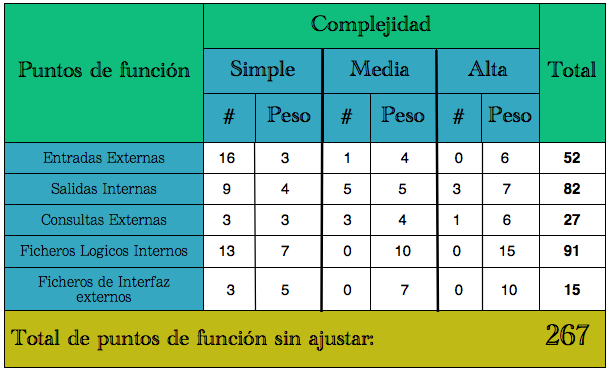
\includegraphics{PFsinAjustar}} 
\vspace{0.35cm}

	Por tanto tenemos un total de 267 puntos de función sin ajustar. Ahora procedemos a calcular el factor de ajuste.

\section{Cálculo del factor de ajuste}
	Existen catorce factores de complejidad, y a cada uno de ellos se le asocia un grado de influencia, entre cero y cinco:
	\begin{itemize}
	\item{\textbf{0:}} Sin influencia. 
	\item{\textbf{1:}} Influencia mínima.
	\item{\textbf{2:}} Influencia moderada.
	\item{\textbf{3:}} Influencia moderada.
	\item{\textbf{4:}} Influencia significativa.
	\item{\textbf{5:}} Influencia apreciable.
	\end{itemize}
	
	\textbf{1} \textbf{Comunicación de datos:} 2, ya que utiliza entrada y salida con impresión remotos (por ejemplo para que los cocineros vean lo que tienen que hacer).
	
	\vspace{0.15cm}
 
	\textbf{2} \textbf{Proceso distribuido:} 0, ya que no existen.
	
	\vspace{0.15cm}
 
	\textbf{3} \textbf{Objetivos de rendimiento:} 1, porque no estamos con un sistema crítico, pero hay requisitos de rendimiento para soportar varias operaciones con un mínimo de eficiencia.
	
	\vspace{0.15cm}
 
	\textbf{4} \textbf{Integración de la aplicación:} 2, pues debe de responder en la tablet o equipo correspondiente aunque haya más aplicaciones abiertas. Además tiene restricciones de seguridad, no todos los empleados pueden ver toda la información del sistema.
	
	\vspace{0.15cm}
 
	\textbf{5} \textbf{Tasa de transacciones:} 3. Habrá horas punta (como la comida), en las que haya más transacciones de información.
	
	\vspace{0.15cm}
 
	\textbf{6} \textbf{Entrada de datos interactiva:} 5, ya que más del 30\% de las entradas son interactivas.
	
	\vspace{0.15cm}
 
	\textbf{7} \textbf{Eficiencia para el usuario final:} 3. Hay más de seis factores, seleción de datos de la pantalla, pantallas con muchos campos y colores, ventanas pop-up, efecto scroll, uso de ratón (en ordenadores), menús...
	
	\vspace{0.15cm}
 
	\textbf{8} \textbf{Actualizaciones interactivas:} 5. Como hemos dicho, al menos una vez por minuto se deben guardar las modificaciones que el usuario haga para evitar la pérdida de información por apagones o agotamiento de batería.
	
	\vspace{0.15cm}
 
	\textbf{9} \textbf{Lógica de proceso interna compleja:} 1, ya que no lleva una lógica muy complicada,  pero hay sistema de seguridad.
	
	\vspace{0.15cm}
 
	\textbf{10} \textbf{Reusabilidad del código:} 4. En principio, con pocas modificaciones de código se podría adaptar para otra empresa hostelera.
	
	\vspace{0.15cm}
 
	\textbf{11} \textbf{Conversión e instalación:} 1, ya que no se defininen requisitos especiales para la instalación, pero tiene que cumplir unas características para que sea sencillo.
	
	\vspace{0.15cm}
 
	\textbf{12} \textbf{Facilidad de operación:} 4. Se presta gran atención al diseño, convirtiéndola en una aplicación vistosa pero sencilla, fácil de aprender a manejar. En posteriores documentos se profundizará en esto. 
	
	\vspace{0.15cm}
 
	\textbf{13} \textbf{Instalaciones múltiples:} 4, ya que se planea al menos tres plataformas (iOS, Android y Windows) con distinto hardware (tablets, smartphones  computadora) y también se documenta.
	
	\vspace{0.15cm}
 
	\textbf{14} \textbf{Facilidad de cambios:} 4. Consultas flexibles del usuario: medias (condiciones lógicas sobre más de un fichero lógico), y el cambio de parámetros de la aplicación con tablas ajenas al código es interactivo.


\vspace{0.35cm}

	En la siguiente tabla se resume el cáculo del factor de complejidad total:

\vspace{0.35cm}

		\begin{tabular}{|p{1cm}||p{8cm}||p{4cm}|}
			\hline
			\textbf{Id.} & \textbf{Factor de complejidad} & \textbf{Grado de influencia} \\ \hline \hline
			\textbf{1} & \textbf{Comunicación de datos} & 2 \\ \hline 
			\textbf{2} & \textbf{Proceso distribuido} & 0 \\ \hline 
			\textbf{3} & \textbf{Objetivos de rendimiento} & 1 \\ \hline 
			\textbf{4} & \textbf{Integración de la aplicación} & 2 \\ \hline 
			\textbf{5} & \textbf{Tasa de transacciones} & 3 \\ \hline 
			\textbf{6} & \textbf{Entrada de datos interactiva} & 5 \\ \hline 
			\textbf{7} & \textbf{Eficiencia para el usuario final} & 3 \\ \hline 
			\textbf{8} & \textbf{Actualizaciones interactivas} & 5 \\ \hline 
			\textbf{9} & \textbf{Lógica de proceso interna compleja} & 1 \\ \hline 
			\textbf{10} & \textbf{Reusabilidad del código} & 4 \\ \hline 
			\textbf{11} & \textbf{Conversión e instalación} & 1 \\ \hline 
			\textbf{12} & \textbf{Facilidad de operación} & 4 \\ \hline 
			\textbf{13} & \textbf{Instalaciones múltiples} & 4 \\ \hline 
			\textbf{14} & \textbf{Facilidad de cambios} & 4 \\ \hline 
		\end{tabular}
\vspace{0.35cm}

	Por tanto el factor de complejidad total o FCT es 39.

	Finalmente, estamos en condiciones de calcular el factor de ajuste o AF:
	
	$$AF = FCT \cdot 0.01 + 0.65 \Rightarrow AF = 39 \cdot 0.01 + 0.65 = 1.04$$

\section{Cálculo de los PF ajustados}
	Al fin, estamos en condiciones de calcular los puntos de función ajustados (PFA)

	$$ \boxed{PFA = PFSA \cdot AF = 267 \cdot 1.04 = 277.7}$$

	, siendo PFSA los puntos de función sin ajustar.
	

\newpage
\mbox{}
\thispagestyle{empty}						% Hoja en blanco, sin numeros ni nada
\newpage
\setcounter{section}{0}

\part{Estimaciones de esfuerzo, coste y duración} %%% PARTE 2 %%%__________________________________________________________
\section{Iniciando la herramienta}
Para esta parte, como se dijo en el \textit{Extracto}, se ha utilizado la herramienta \texttt{COCOMO II.2000.4}.

En primer lugar, se introdujo un nuevo módulo: \textit{Hostelería}. Posteriormente, en \textit{Module size} se añadió los datos sobre PF. El peso de cada uno es el habitual, seleccionado así:

\vspace{0.35cm}
\hspace{3.5cm}
\scalebox{0.45}{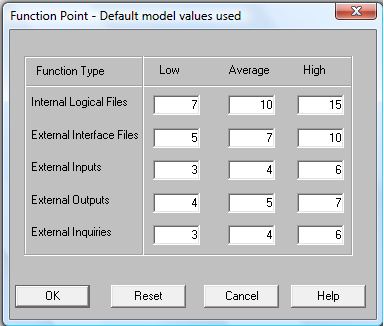
\includegraphics{PFCOCOMOpeso}} 
\vspace{0.35cm}

El número de entradas, salidas etc. exactamente igual que antes:

\vspace{0.35cm}
\hspace{2.9cm}
\scalebox{0.5}{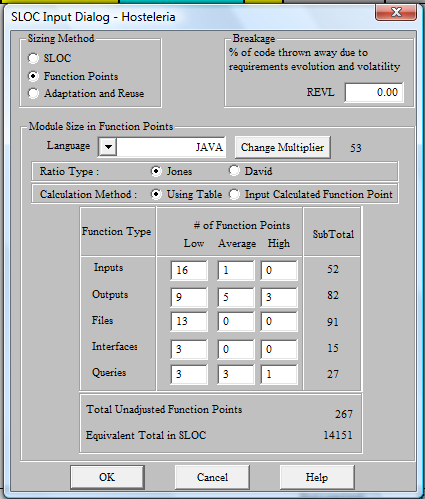
\includegraphics{PFCOCOMO}} 
\vspace{0.35cm}

Con ello obtenemos una medida del tamaño de la aplicación. Nos da 14151 líneas de código.

\section{Factores de escala (Scale Factor)}
\begin {itemize}
	\item {PREC: Precedentness}

	El equipo de desarrolladores está compuesto por principiantes poco acostumbrados a trabajar con sistemas software, por tanto consideramos que este campo debe ser \textit{muy bajo}.
	\item {FLEX: Development Flexibility}

	La flexibilidad de desarrollo se fija como \textit{baja} ya que hay unos requisitos predefinidos y que estamos trabajando con  el Proceso Unificado.
	\item {RESL: Architecture/Risk Resolution}

	El estudio de los riesgos se puede examinar en el documento de \texttt{Gestión de riesgos Software}, donde se ve que tenemos 5 riesgos con un nivel intolerable. Debido a esto y a la arquitectura, fijamos este valor como \textit{bajo}.
	\item {TEAM: Team Cohesion}

	Ya que los miembros del equipo se conocen bien, hay buen ambiente de trabajo y se ven prácticamente todos los días, consideramos que la cohesión del equipo es \textit{alta}. Además, se tiene bastante capacidad de acomodación a los intereses de otros stakeholders.
	\item {PMAT: Process Maturity}

	Mirando el CMM Maturity Model hemos concluido que el proyecto se encuentra en un nivel 2, que es una madurez media. Por lo tanto queda como \textit{nominal}.
\end{itemize}

Con estos datos, la herramienta determina que el factor de escala es 22.77, como se ve en la imagen.

\vspace{0.4cm}
\hspace{3cm}
\scalebox{0.9}{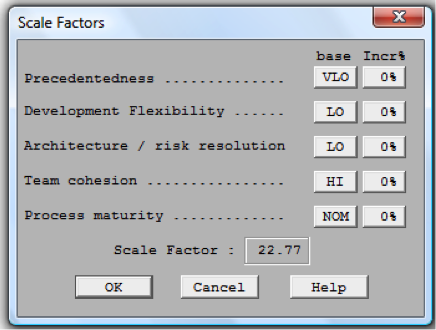
\includegraphics{sf}} 
\vspace{0.35cm}

\section{Factor de ajuste del esfuerzo (EAF)}
\begin {itemize}
	\item{Factores del producto}
		\begin{itemize}
			\item{RELY: Required Software Reliability}

			El software debe tener una fiabilidad \textit{alta}, sobre todo si se trata de una empresa mediana- grande.
			\item{DATA: Data Base Size}

			Ya que se manejan bases de datos de clientes, empleados y platos, y que de nuevo cuanto más grande sea el negocio más crecen estas bases de datos, se fija como \textit{alta}.
			\item{CPLX: Product Complexity}

			\textit{Baja}, ya que aunque sea un software bastante grande, no es complejo ni tiene elementos sofisticados.
			\item{RUSE: Required Reusability}

			Se pretende que pueda ser adaptable con pocas modificaciones a distintos clientes, por lo que la reusabilidad es \textit{muy alta}.
			\item{DOCU: Documentation Match to Life-Cycle Needs}

			\textit{Nominal}, no es determinante.
		\end{itemize}
	\item{Factores de la plataforma}
		\begin{itemize}
			\item{TIME: Execution Time Constraint}

			\textit{Nominal}, ya que no estamos trabajando con sistemas críticos o similares.
			\item{STOR: Main Storage Constraint}

			\textit{Nominal} por el mismo motivo.
			\item{PVOL: Platform Volatility}

			\textit{Nominal}.
		\end{itemize}
	\item{Factores de personal}
		\begin{itemize}
			\item{ACAP: Analyst Capability}

			Ya que los integrantes del grupo tienen conocimientos fuera de la informática también, se considera que tienen una \textit{alta} capacidad de análisis.
			\item{PCAP: Programmer Capability}
	
			Al tratarse de estudiantes todavía no se tienen unos conocimientos extensos de progamación, por lo que consideramos esta campo como \textit{bajo}.
			\item{AEXP: Application Experience}

			\textit{Nominal}.
			\item{PEXP: Platform Experience}

			\textit{Nominal}.
			\item{LTEXT: Language and Tool Experience}

			\textit{Alta} porque trabajamos con Java en un entorno al que estamos acostumbrados: Eclipse. La otra herrmaienta que utilizamos la mayor parte del tiempo es el TeXworks para escribir en \LaTeX, que también la dominamos bastante.
			\item{PCON: Personnel Continuity}

			\textit{Alta} salvo abandono.
		\end{itemize}
	\item{Factores del proyecto}
		\begin{itemize}
			\item{TOOL: Use of Software Tools}

			\textit{Bajo} ya que apenas se utilizan herramientas.
			\item{SITE: Multisite development}

			\textit{Bajo}, ya que como se ha dicho antes, los integrantes del grupo se ven prácticamente todos los días.
		\end{itemize}
\end{itemize}

Con estos datos, el COCOMO II determina un factor de ajuste del esfuerzo de 1.19, como se puede ver en la figura.

\vspace{0.35cm}
\hspace{3cm}
\scalebox{0.9}{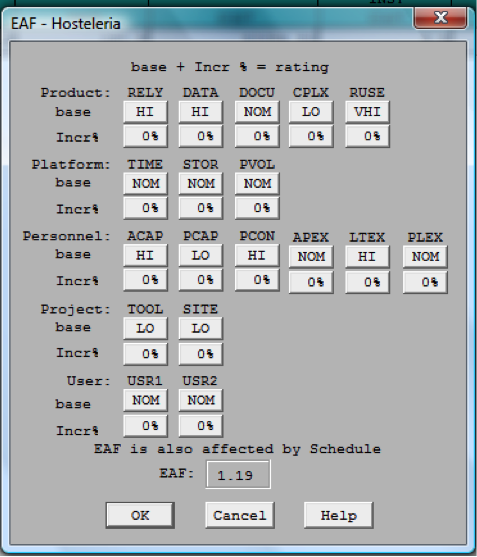
\includegraphics{eaf}} 
\vspace{0.35cm}

\section{Esfuerzo, coste  duración}
También se detalló el salario en dólares por mes (que aparece como \textit{LABOR RATE (\$/month)}). Suponiendo un salario humilde, estimamos unos 700 \$/mes. Además, añadimos el lenguaje de programación elegido: Java, como ya hemos dicho en varias ocasiones. 


\vspace{0.35cm}
\hspace{-3.2cm}
\scalebox{0.8}{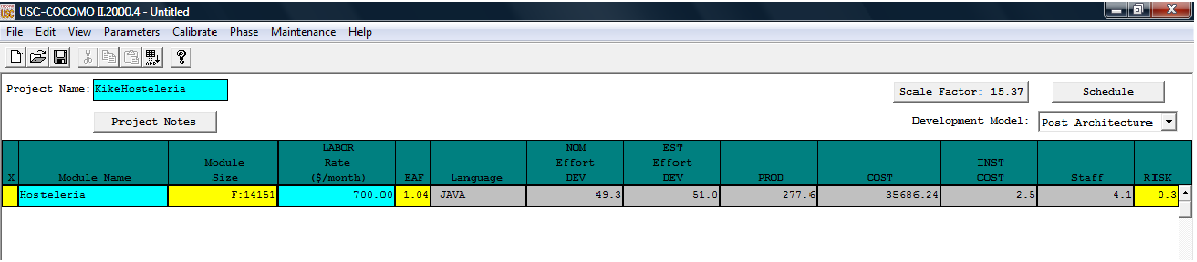
\includegraphics{COCOMOTODO2}} 
\vspace{0.35cm}

Tras todas estas consideraciones, el programa nos da las estimaciones:

\vspace{0.35cm}
\hspace{-3.2cm}
\scalebox{0.85}{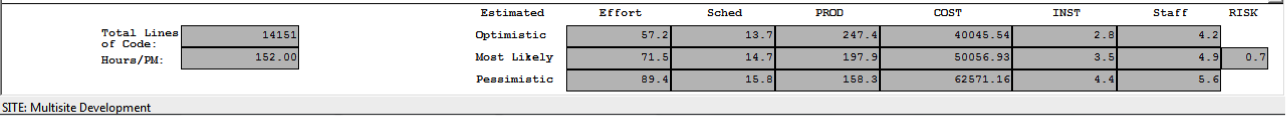
\includegraphics{COCOMOTODO1}} 
\vspace{0.35cm}

\begin{itemize}
	\item{\bfseries{Estimación de esfuerzo:}}
	Según la herramienta, lo más probable es que se necesiten \textbf{\underline{71.5 personas · mes}}, aunque el valor optimista es de 57.2 y el pesimista de 89.4, conviertiéndolo en un proyecto de envergadura media.
	\item{\bfseries{Estimación de coste:}}
	La estimación del coste, como hemos comentado antes, está hecha con un supuesto de un salario de 700 \$/mes, aunque esto son sólo conjeturas ya que se trata de un proyecto académico. Así, salen \textbf{\underline{50056.93 dólares}}, que son 38.544,637 euros. Además, se puede apreciar que se estima un precio de unos 3.5 \$ por cada instrucción de la aplicación.
	\item{\bfseries{Estimación de duración:}}
	Según el COCOMO II, durará \textbf{\underline{14.7 meses}}, poco más de un año, entre 13.7 y 15.8 meses en el mejor y peor caso respectivamente. Es interesante ver que si dividimos el esfuerzo entre el tiempo obtenemos el número aproximado de personas que son necesarias cada mes, y en nuestro caso es 4.86, es decir unas 5 personas cada mes, justo el número de miembros del equipo.
\end{itemize}

\textbf{\underline{Nota:}} Lo que aparece entre la duración y el coste en la herramienta es la productividad, que se obtiene de dividir SLOC entre el esfuerzo más probable, y obtenemos que es 197.9 SLOC/pm.

\newpage
\mbox{}
\thispagestyle{empty}						% Hoja en blanco, sin numeros ni nada al final del documento
\newpage

\end{document}